%!TEX root = ../Main.tex
Ever since its isolation and initial characterisation, graphene has been widely researched for potential applications. [Insert litt.] On a more recent timescale so called nano-porous graphene devices (NPGs) has been proposed for various applications. [Insert litt.] These devices are made up of single layered graphene with periodic holes (hence the porous) with which the intact graphene constitutes ribbons and bridges in the structures. Because of graphenes electrical properties [Insert litt], one should be able to finely control the electron currents in the devices and thus create nanometer circuits for use as e.g. chemical detectors. Because of its novelty, the fabrication of such devices are limited. It is first considered for fabrication and practical testing when theoretical simulations shows promising results. Common simulation tools for the electron transport in simple devices (albeit in large scales) are those from the SIESTA project (TBtrans), whith results analysed using SISL\cite{zerothi_sisl}. SIESTA generally deal with DFT calculations, which can be extrapolated using tight-binding for larger scales\cite{calogero_electron_2019}. However DFT programs run complex calculations and might seem as a blackbox for non-physcisists. In order to better understand electron transport this project deals with a simpler approach to electron transport using only tight-binding by developing a set of tools in Python, using NumPy and numerical calculations. We utilise Greens functions and a very efficient recursion formula to gather transmission plots and band structure plots for various NPGs, whilst comparing our results with those obtained by classical DFT programs. The main scope is the development of the tight-binding scripts, comparing results with those of DFT calculations and discuss whether a clean tight-binding approach can sufficiently be used for the relatively simple NPGs.
To summarise:
\begin{itemize}
    \item Apply quantum mechanics for electron transport in NPGs.
    \item Use numerical methods (recursion algorithms, linear algebra) with NumPy to implement tight-binding.
    \item Calculate band structures and transmission plots for various devices.
    \item Gather single-particle Green’s functions and LDOS of said devices.
\end{itemize}
The report is organised on the following way:
\begin{enumerate}
    \item \cref{theorysec,hamilsec,greensec,transec} deals with the development of our methodology.
    \item \cref
\end{enumerate}
The code repository (which also includes the \latex files for this report) can be found on Github: \faGithub \ \url{https://github.com/rwiuff/QuantumTransport}


%!TEX root = ../Main.tex
The conclusion of the preliminary work revolves around the Transmission Routine. Here all the functions producing on-site Hamiltonians, full Hamiltonians, hopping matrices, band structures, self energy and Green's functions by recursion play their part in getting the transmission through the material. \textit{This part is an attempt to describe the basic theory behind transmission/transport and it is very likely to need rework, additions and editing} The transmission tells us the probability whether an electron will be transported trough all the possible \(\pi\)-orbitals in a "device region" at different energies and thus how the "device region" affects the overall current through larger systems. This means that the system will have to be well defined before one can use the functions developed for calculation of the different parts needed for production of transmission. The "device region" contains at least one central unit cell as well as a "left" and "right" unit cell. The left and right unit cell represents the contact region of the device i.e. the two parts that connects to the "rest" of the system/molecule. It is assumed that the "rest of the molecule" represent a system that is made up of unit cells which can be reduced by recursion, though not necessarily identical on each side (left and right). Knowing which "blocks" the system contains and how to obtain them with the already developed functions, three main ingredients are needed to obtain the transmission through a device. The first one is the Green's function for the device region \(\mathbf{G}_D\). The device region of cause includes the device Hamiltonian \(\mathbf{H}_D\) and in addition, \(\mathbf{H}_D\) contfor which one needs the device Hamiltonian \(\mathbf{H}_D\) as well as the left and right selfenergies \(\mathbf{\Sigma}_L, \ \mathbf{\Sigma}_R\). The left and right selfenergies constitutes the second ingredient and can be obtained through left and right hopping matrices as well as the left and right on-site Green's functions. The last main ingredient are \(\mathbf{\Gamma}_L,\ \mathbf{\Gamma}_R\) which are matrix operators describing the coupling between the left and right parts of Hilbert space. They are called rate equations because..... The rate equation are obtained via the self energies in the following fashion: 
\begin{align}\label{rateeq}
\mathbf{\Gamma}_{L/R} = i(\mathbf{\Sigma}_{L/R} - \mathbf{\Sigma}^{\dagger}_{L/R})
\end{align}To give an overview of how the different matrices are defined in relation to a system an illustration has been made. See \cref{systemillu}. Using the Green's function, left/right self energies as well as the left/right rate matrices, the transmission, as a function of energy, can be obtained via the following equation:
\begin{align}
    T(E) = \text{Tr}[\mathbf{\Gamma}_R\mathbf{G}_D\mathbf{\Gamma}_L\mathbf{G}_D^{\dagger}](E)
    \label{transeq}
\end{align}
Where Tr is the trace of the matrix product. 
\begin{figure}
    \centering
    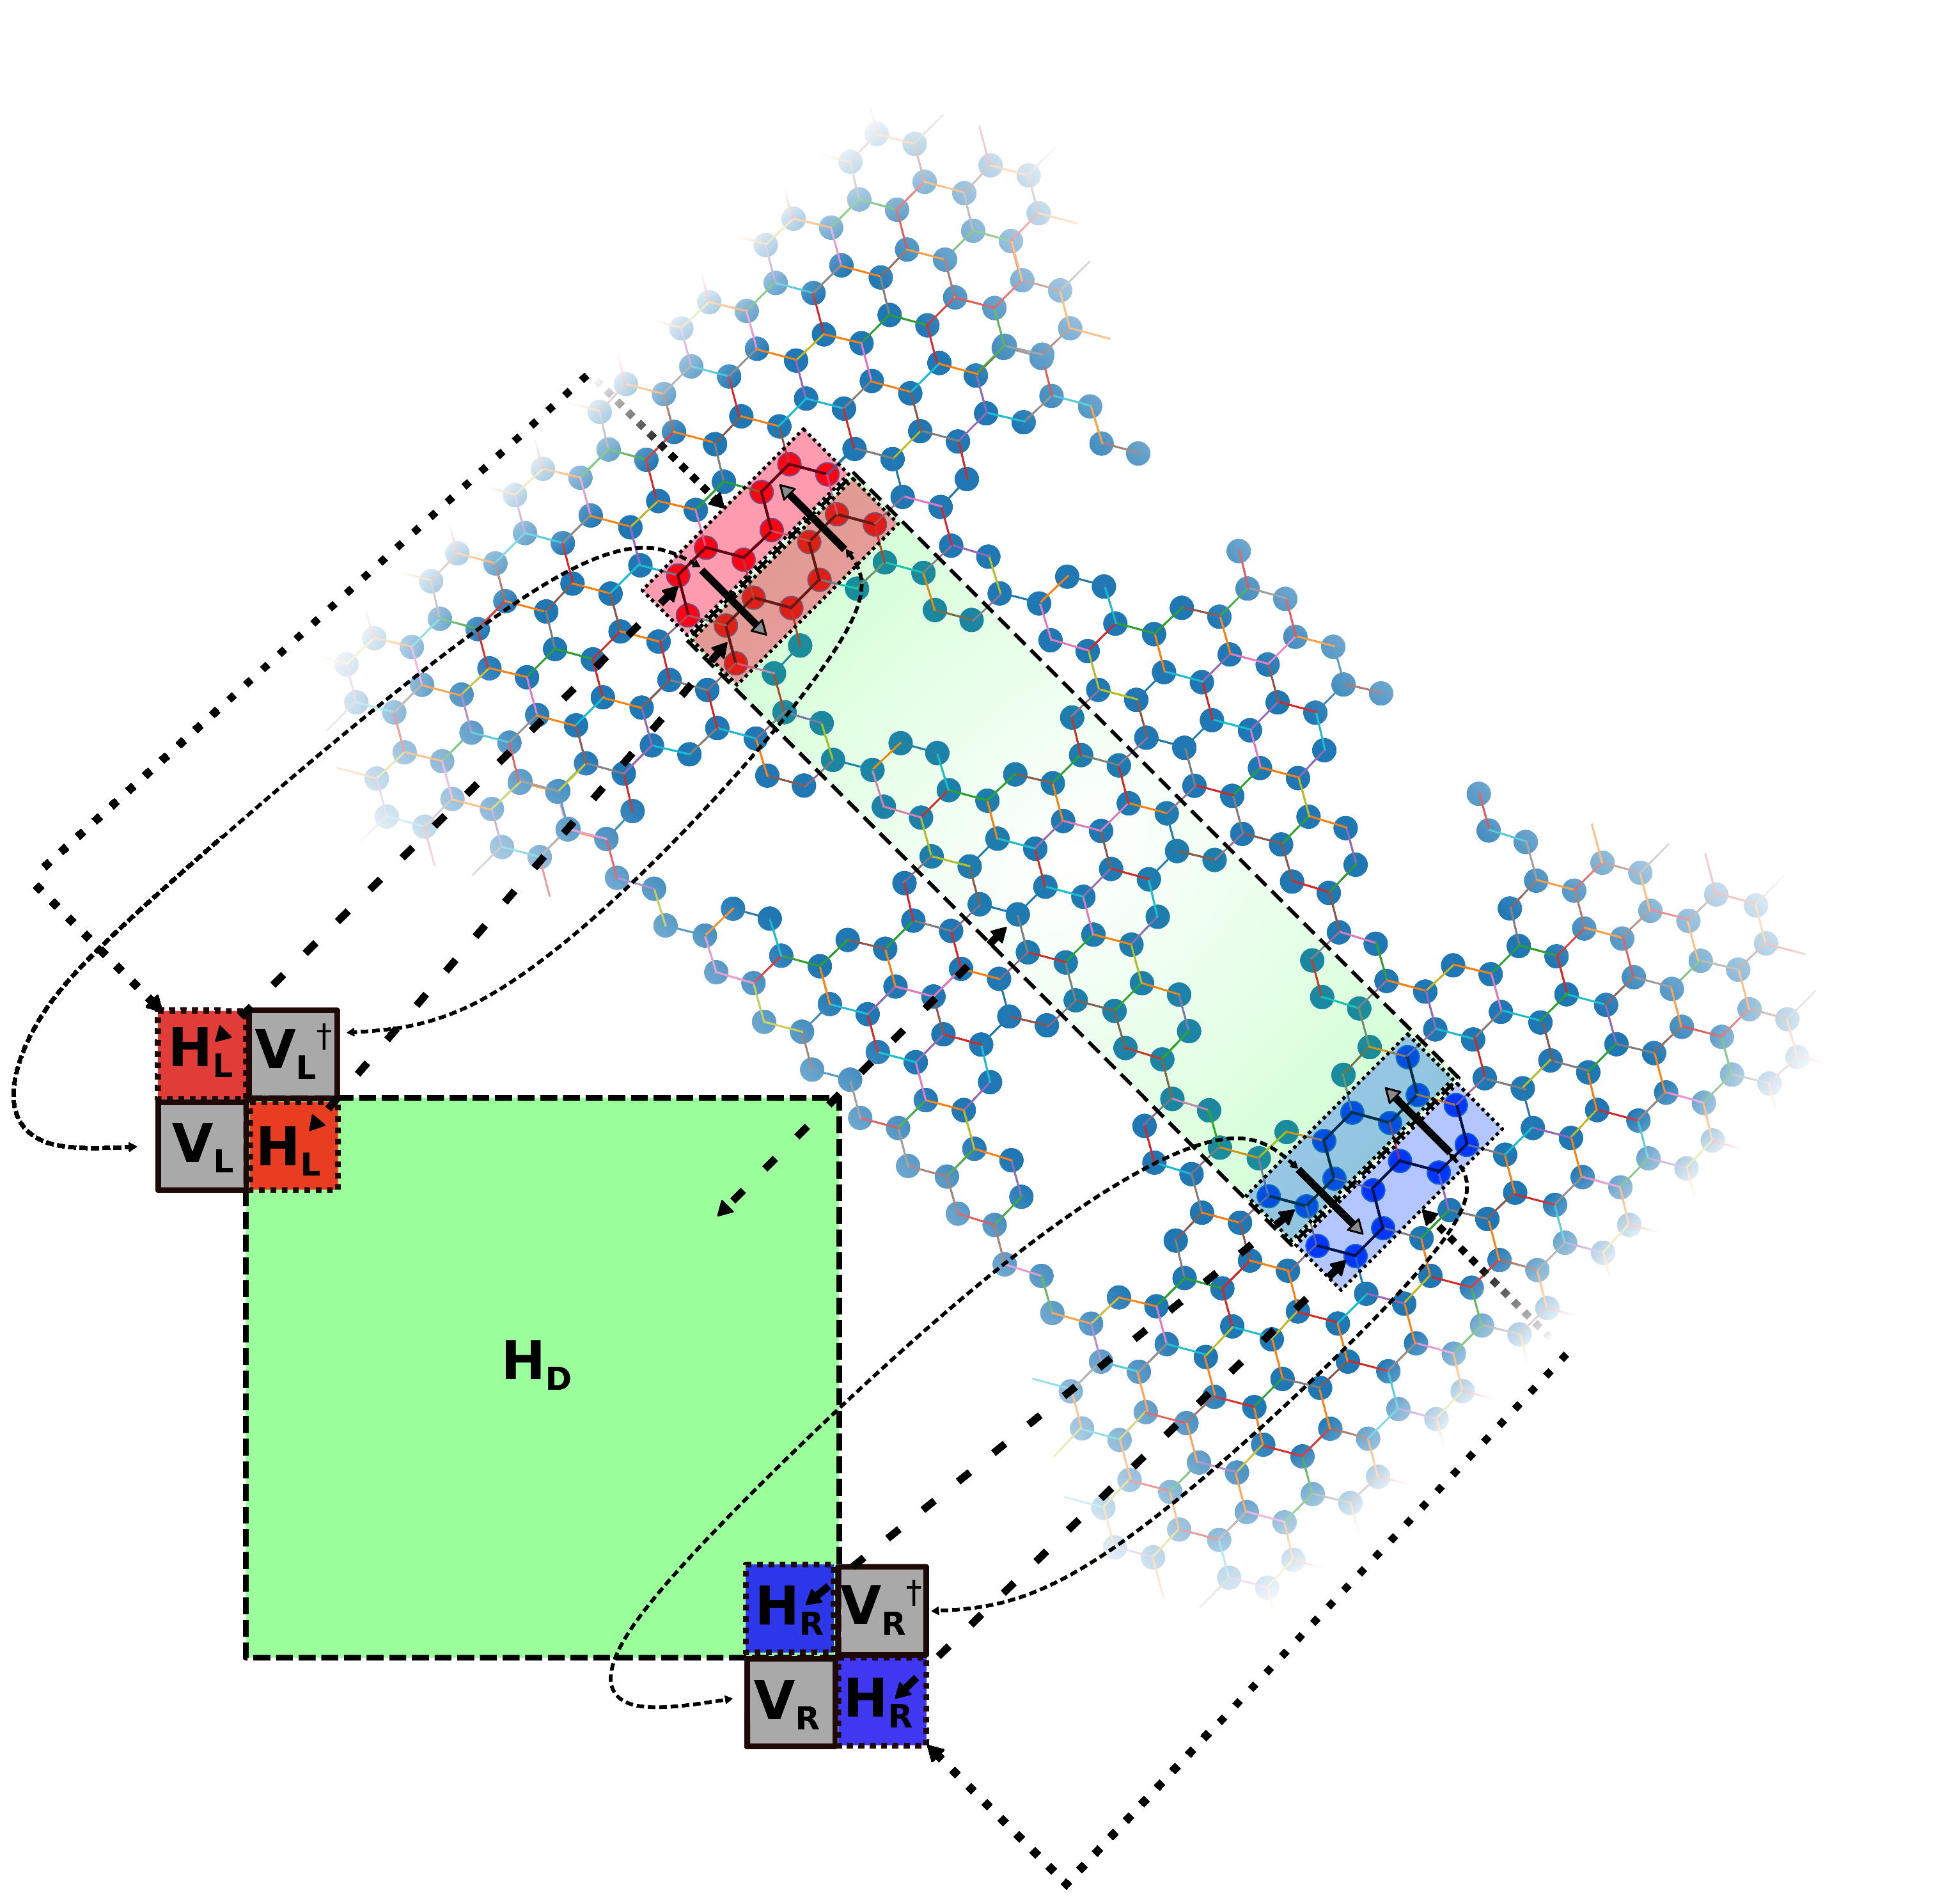
\includegraphics[width=0.9\textwidth]{Figures/illu.eps}
    \caption{Illustration showing how the different parts of the system are translated into matrix blocks. On the graphene the green box is the unit cell of the device. It includes one red and blue box which themselves are unit cells of the left and right contacts. These unit cells can be translated into Hamiltonian matrices \(\textbf{H}_D, \ \textbf{H}_L,\ \textbf{H}_R\) as illustrated. Note that because the first of the left and right unit cells (red and blue) are inside the device (green region), they can be picked out of \(\textbf{H}_D\) directly and so it is not necessary to make them from scratch. The two other unit cells lying outside the device region represents what could be an infinite contact region. The contact region is therefore potentially of an infinitely bigger dimension compared to the device region, however, by recursion, this region can be collapsed into a single Hamiltonian of same dimension as the one inside the device region. Finally the two fat black arrows (not dotted) on each side of the device represents the hopping between the device and contact region. Note that the direction of hopping corresponds to a specific hopping matrix. F.ex. left-to-right is the ordinary hopping matrix while right-to-left is its conjugate (for both left and right side of the device).}
    \label{systemillu}
\end{figure}
\subsubsection{Transmission in 1D a simple example}
As with the Recursion Routine, the development of this routine will be build up around a small system in order to make sure that the obtained results are as expected, thereafter generalising the routine to suit all kinds and sizes of system. First thing is to define the device in the same manner as \cref{systemillu} so that the device Hamiltonian \(\textbf{H}_D\) can be obtained through the already defined function \textit{Onsite}. The left and right Hamiltonian \(\textbf{H}_{L/R}\) are thus picked out as described in \cref{systemillu}. A smart function has been implemented in order to allow the user to choose the left and right contact cells using indices given to each atom in the system of choice (See \cref{basicstructurewithcontacts} for an example).
\begin{figure}
\begin{subfigure}[b]{0.4\textwidth}
		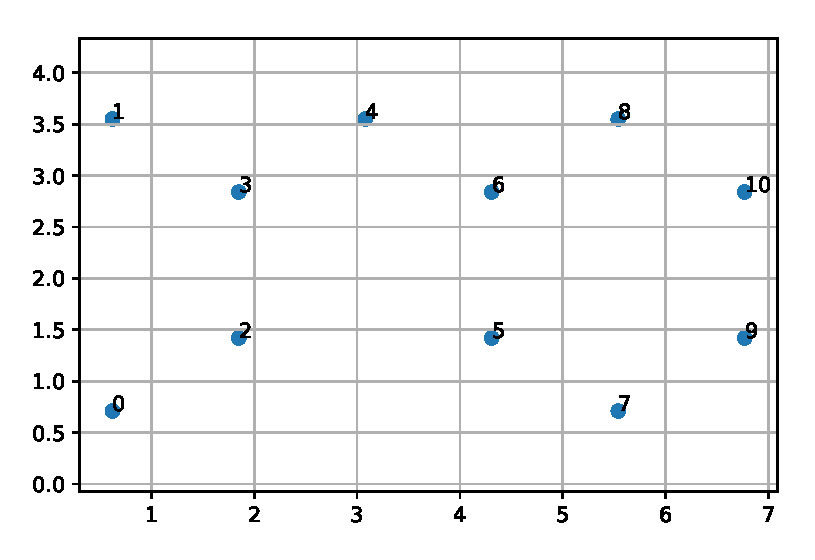
\includegraphics[width=\textwidth]{Figures/basicstructure.eps}
		\caption{The basic structure plotted with indices\vspace{\baselineskip}}
		\label{basicstructure}
	\end{subfigure}\vspace{2mm}
	~ %add desired spacing between images, e. g. ~, \quad, \qquad, \hfill etc.
	%(or a blank line to force the subfigure onto a new line)
	\begin{subfigure}[b]{0.4\textwidth}
		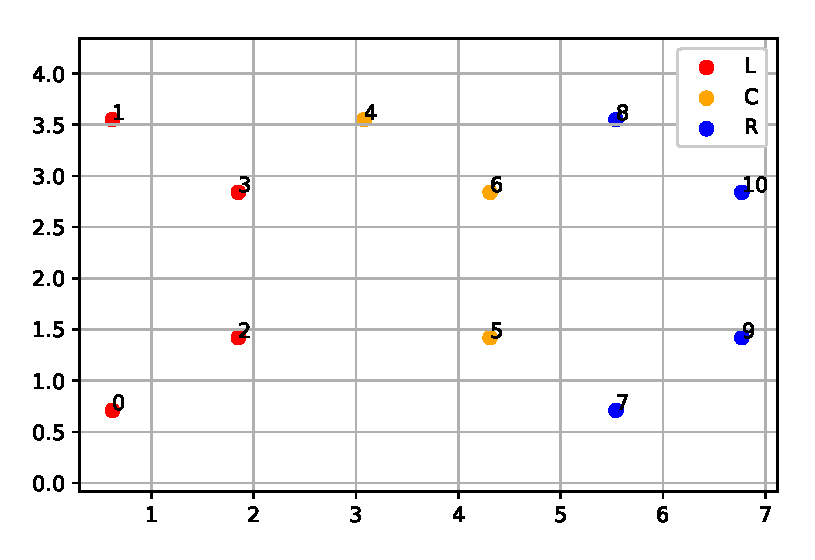
\includegraphics[width=\textwidth]{Figures/basicstructurewithcontacts.eps}
		\caption{The same structure now shown with indices marked red and blue as per users choice of contact atoms}
		\label{basicstructurewithcontacts}
	\end{subfigure}
	\caption{Figure showing the interface integrated into the script.}\label{interface}
\end{figure}
This allows the user to get the dimensions needed to define the left and right Hamiltonians so they can be picked out of the device Hamiltonian. From the left and right Hamiltonian the corresponding hopping matrices are defined using the \textit{Hop} function. Then the \textit{EnergyRecursion} is used to obtain the Green's function for the device. This function is a more elaborate version of the earlier mentioned \textit{RecursionRoutine}. It uses the old recursion routine to calculate the self energies for the left and right cells (\(\mathbf{\Sigma}_{L/R}\)) (see line 164-165 \cref{engrec}) and then uses those to calculate the device Green's function \(\textbf{G}_D\) as well as the left and right rate matrices \(\mathbf{\Gamma}_{L/R}\), using the equations \cref{rateeq}, \cref{devicegreens} (see \cref{engrec} line 176-179).\im{Listings/Functions.py}{156}{185}
\vspace{-1\baselineskip}
\captionof{listing}{lalala\label{engrec}}\vspace{\baselineskip}The output of the energy recursion function is the two rate matrices (left and right) as well as the device Green's function and as per \cref{transeq} the matrices needed for transmission have been obtained. As seen in \cref{transfunc} the transmission function \textit{Transmission} simply carries out the matrix product and subsequent trace of the resulting matrix and outputs a range of transmission probabilities which is then plotted against an energy range. Do mind that this is still just 1D in the sense that the transmission only moves in one direction. A plot of the transmission for such a simple 1D system (the one in \cref{basicstructure}) can be seen in \cref{alphatrans}.\im{Listings/Functions.py}{188}{195}
\vspace{-1\baselineskip}
\captionof{listing}{lalala\label{transfunc}}\vspace{\baselineskip}
\begin{figure}[ht]
    \centering
    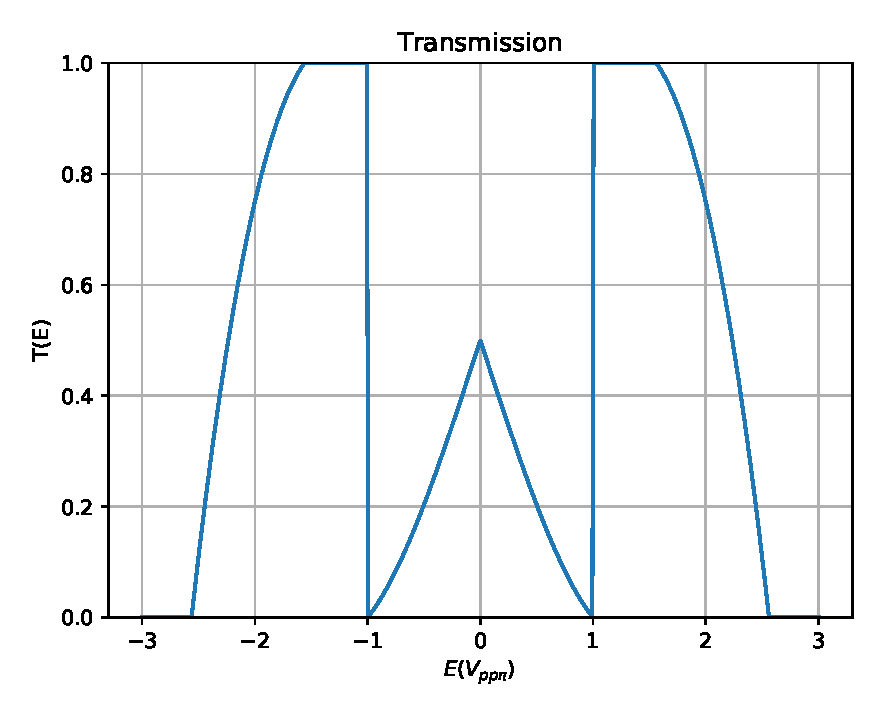
\includegraphics[width =0.5\textwidth]{Figures/alphaTE.eps}
    \caption{Transmission plot for the system in \cref{interface}}
    \label{alphatrans}
\end{figure}
\subsubsection{Development of transmission to 2D}
Lastly the transmission routine needs to be generalised so it can handle transport in two directions. The most convenient approach is to work with five real space unit cells as a starting point. One center cell, a right and a left cell representing the contacts and then two additional cells on the left and right, representing the rest of the contact region. This would be the minimum amount of cells needed to generalise the transmission. One might have more center cells if the structure changes from one of those cells to the other. First these five unit cells will be defined using already developed tools. Then a big Hamiltonian, including all coordinates from the five cells representing real space are created, again using existing functions. One could call this big Hamiltonian \(\textbf{H}_{\text{Bigreal}}(xyz_0,xyz_0)\). It is a function of two sets of identical coordinates, namely the ones used to create the Hamiltonian itself. This has also been the case for all previous calculations, but the following steps will make it clear why it is explicitly stated for this Hamiltonian. The left/right on-site Hamiltonians and hopping matrices can thus be picked out of \(\textbf{H}_{\text{Bigreal}}(xyz_0,xyz_0)\) as before to get the Green's functions, self energies for transmission in real space, just as in the previous section. But instead, before the Green's function, self energies and transmission is calculated, the left/right onsite-Hamiltonian as well as their hopping matrices are defined as functions of a variable \(k\) and the hopping will additionally have a phase added which depends on a variable \(q\). As an example the following is the equation for the full right side Hamiltonian using the right on-side Hamiltonian with its hopping matrices: \(\textbf{H}_R(k,q) = \textbf{V}_R(k)e^{iq}+\textbf{V}^{\dagger}_R(k)e^{-iq}+\textbf{h}_R(k)\). The \(k\) represents .... and the \(q\) represents ..... The next part is to obtain
the hop from \(\textbf{H}_{\text{Bigreal}}(xyz_0,xyz_0)\) to an equal cell in the other (transverse) direction, so that the transmission will become truly 2D. Firstly the hopping between \(\textbf{H}_{\text{Bigreal}}(xyz_0,xyz_0)\) and a transversely shifted Hamiltonian is defined as \(\textbf{W} = \textbf{H}_{\text{Bigtrans}}(xyz_0,xyz_1)\) (Here using \textbf{W} as not to confuse it with \textbf{V} which is hopping between cells in real space). Note that the index of one of the coordinate sets have changed to 1. This corresponds to a shift by the lattice vector going in the transverse direction to that of the transmission direction defined in 1D. With the hopping matrices for the transverse direction defined a Hamiltonian dependent on \(k\)-point values can be defined as:\begin{align}
    \textbf{H}(k) &= \textbf{h}+\textbf{W}e^{ik}+\textbf{W}^{\dagger}e^{-ik}\\
    &= \textbf{H}_{\text{Bigreal}}(xyz_0,xyz_0) + \textbf{H}_{\text{Bigtrans}}(xyz_0,xyz_1)e^{ik}+\textbf{H}_{\text{Bigtrans}}^{\dagger}(xyz_0,xyz_1)e^{-ik}
\end{align}
Now a Hamiltonian, dependent of a variable \(k\) has been defined, and thus it is now possible to get self energies, Green's functions that is \(k\)-dependent as well as a transmission (also \(k\)-dependent) which can be found for different \(k\)-points i.e. different points in the transverse direction (inverse space). This hereby concludes the all the initial effort to develop a code which can do calculations of different points of interest (Green's function plots, band structures and transmission) in a two dimensional material such as NPG. Following is a walk through as to how this last step has been implemented through code programming. 

\section{Exploring functionality of GNR bridges}\label{testsec}